\documentclass{patmorin}
\listfiles
\usepackage{amsthm,amsmath,graphicx}
\usepackage{pat}
%\usepackage{coffee4}
\usepackage[letterpaper]{hyperref}
\usepackage[dvipsnames]{color}
\definecolor{linkblue}{named}{Blue}
\hypersetup{colorlinks=true, linkcolor=linkblue,  anchorcolor=linkblue,
citecolor=linkblue, filecolor=linkblue, menucolor=linkblue, pagecolor=linkblue,
urlcolor=linkblue, pdfcreator=Me, pdfproducer=Me} \setlength{\parskip}{1ex}
\usepackage{tikz}

\newcommand{\lstlabel}[1]{\label{lst:#1}}
\newcommand{\lstref}[1]{Listing~\ref{lst:#1}}
\newcommand{\Lstref}[1]{\lstref{#1}}

\DeclareMathOperator{\block}{block}
\newcommand{\naive}{na\"{\i}ve}


\title{\MakeUppercase{New Bounds for Facial Non-Repetitive Colouring}\thanks{This research is partially funded by NSERC.}}

\author{Prosenjit Bose,\, Vida Dujmovi\'c,\, Pat Morin,\, Lucas Rioux Maldague}



\begin{document}
\maketitle


\begin{abstract}
  We prove that the facial non-repetitive chromatic number of any outerplanar graph is at most 11 and of any planar graph is at most 22.
\end{abstract}


\section{Introduction}

\section{Preliminary Results and Definitions}

A graph is \emph{$k$-connected} if it contains more than $k$ vertices and has
no vertex cut of size less than $k$.  A \emph{$k$-connected component} of a graph $G$ is a maximal subset of vertices $G$ that induces a $k$-connected subgraph.

A \emph{plane graph} $G$ is a fixed embedding of a graph in the plane such
that its edges intersect only at their endpoints. An \emph{outerplane}
graph $G$ is a plane graph such that all the vertices of $G$ are adjacent
to the outside face of $G$. A \emph{chord} in an outerplane graph is
an edge that is not incident to the outer face. A \emph{cactus graph}
is an outerplane graph with no chords.

A \emph{closed walk} in a graph $G$ is a sequence of vertices
$v_0,\ldots,v_{\ell-1}$ such that, for every $i\in\{0,\ldots,\ell-1\}$
the edge $v_iv_{(i+1)\bmod \ell}$ is in $E(G)$.

A \emph{facial walk} in a plane graph $G$ is a closed walk
$v_0,\ldots,v_{\ell-1}$ such that, for every $i\in\{0,\ldots,\ell-1\}$,
the edges $v_{(i-1)\bmod \ell} v_i$ and $v_iv_{(i+1)\bmod\ell}$ occur
consecutively in the counterclockwise cyclic ordering of the edges
incident to $v_i$ in the embedding of $G$.

A \emph{facial path} is a contiguous subsequence of a facial walk that
is a path in $G$.

A \emph{bridge} in a graph $G$ is an edge whose removal increases the number of connected components in $G$.  A graph is \emph{bridgeless} if it has no bridges.

NOTE: Add induced subgraph notations.

\section{Outerplane Graphs}

Let $G$ be an outerplane graph. A \emph{blocking set} of $G$ is a set
of vertices $B \subseteq V(G)$ such that for each 2-connected component
$H$ of $G$, $H \setminus B$ is a tree and for each inner face $F$,
$F \setminus B \not= \emptyset$.  See Figure \ref{fig:blocking_set}
for an example of a blocking set.

\begin{figure}[!ht]
  \centering
  
  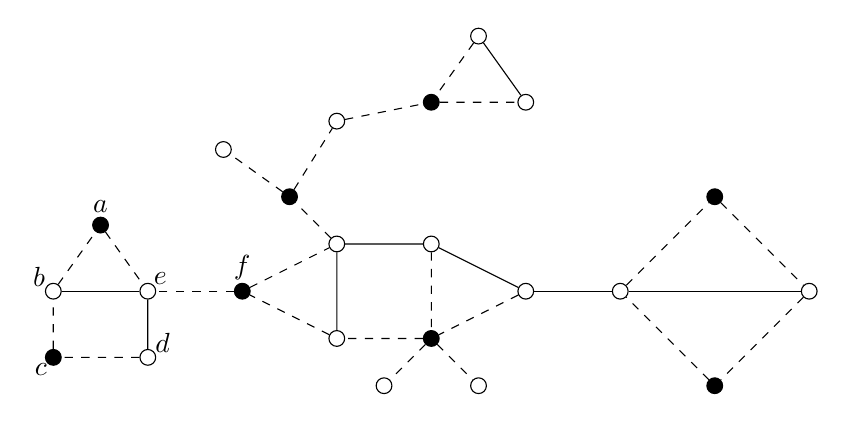
\begin{tikzpicture}[scale=1.2,auto=left]
    
    \begin{scope}[every node/.style={circle,draw=black,fill=white,minimum size=0.2cm, inner sep=0}]
      \node[fill=black,label=91:$f$] (a) at (0,0) {};
      \node[] (b) at (1,0.5) {};
      \node[] (c) at (2,0.5) {};
      \node[] (d) at (3,0) {};
      \node[fill=black] (e) at (2,-0.5) {};
      \node[] (f) at (1,-0.5) {};
      \node[] (g) at (4,0) {};
      \node[fill=black] (h) at (5,1) {};
      \node[] (i) at (6,0) {};
      \node[fill=black] (j) at (5,-1) {};
      \node[label=45:$e$] (k) at (-1,0) {};
      \node[label=45:$d$] (l) at (-1,-0.7) {};
      \node[fill=black,label=-135:$c$] (m) at (-2,-0.7) {};
      \node[label=135:$b$] (n) at (-2,0) {};
      \node[fill=black,label=90:$a$] (o) at (-1.5,0.7) {};
      \node[fill=black] (p) at (0.5,1) {};
      \node[] (q) at (-0.2,1.5) {};
      \node[] (r) at (1,1.8) {};
      \node[] (s) at (1.5,-1) {};
      \node[] (t) at (2.5,-1) {};
      
      \node[fill=black] (u) at (2,2) {};
      \node[] (v) at (3,2) {};
      \node[] (w) at (2.5,2.7) {};
      
      \foreach \from/\to in {b/c,c/d,f/b,
                             d/g,g/i,
                             k/l,k/n,
                             v/w}
	\draw (\from) -- (\to);

      \foreach \from/\to in {a/b,f/a,d/e,e/f,g/h,h/i,i/j,j/g,l/m,m/n,n/o,o/k,
                             b/p,p/q,p/r,c/e,e/t,e/s,a/k,r/u,u/v,w/u}
	\draw[dashed,black] (\from) -- (\to);
    \end{scope}
  \end{tikzpicture}
  \caption{Blocking set $B$ of an outerplane graph $G$, with blocking set vertices denoted in black. In dashed, edges of $G\setminus B$. Notice that, for each 2-connected component of $G$, the vertices of that component in $G\setminus B$ are contained in a single tree.}

  \label{fig:blocking_set}  
\end{figure}

The definition of a blocking set is subtle and implies three properties
that we will use throughout.   An \emph{ear} in
an outerplanar graph is an inner face that is incident to exactly one
chord. An ear is \emph{triangular} if it has three vertices.

\begin{obs}\obslabel{no-chords}
   For any blocking set $B$ of $G$, $B$ does not include both endpoints
   of any chord of $G$.
\end{obs}

\begin{obs}\obslabel{consecutive}
   For any blocking set $B$ of $G$ and any inner face $F$ of $G$, the
   vertices of $V(F)\cap B$ occur consecutively on the boundary of $F$ 
\end{obs}

\begin{obs}\obslabel{non-empty-path}
  For every inner face $F$ of $G$, $F \setminus B$ is a non-empty path.
\end{obs}


\begin{lem}\lemlabel{biconnected}
  For every biconnected outerplane graph, $G$, and any vertex $v\in
  V(G)$, there exists a blocking set $B$ of $G$ such that $v\in B$ and,
  for each inner face $F$ of $G$, $|B\cap V(F)|=1$.
\end{lem}

\begin{proof}
  The proof is by induction on the number of internal faces.  If $G$ has
  only face, we take $B=\{v\}$.  Otherwise, select some ear, $F$ of $G$
  whose chord is $uw$ and such that $v\not\in V(F)\setminus\{u,w\}$.
  Let $G'=G-(V(F)\setminus\{u,w\})$.  The graph $G'$ has one less internal
  face than $G$ so, by induction, it has a blocking set $B'$ that satisfies
  the conditions of the lemma.  There are two cases to consider:
  \begin{enumerate}
    \item If one of $u$ or $w$ is in $B'$ then we take $B=B'$ to obtain
      a blocking set that satisifes the conditions of the lemma.

    \item Otherwise, let $x$ be any vertex in $V(F)\setminus\{u,w\}$ and
      take $B=B'\cup\{x\}$ to obtain a blocking set that satisifes the
      conditions of the lemma. \qedhere
  \end{enumerate}
\end{proof}

\Lemref{biconnected} allows us to prescribe that a particular vertex
$v$ be included in the blocking set, but it will also be convenient to
exclude a particular vertex $v$ by using \lemref{biconnected} to force
the inclusion of $v$'s neighbour on the outer face (which is also on
some inner face with $v$).

\begin{cor}\corlabel{biconnected-out}
  For every biconnected outerplane graph, $G$, and any vertex $v\in
  V(G)$, there exists a blocking set $B$ of $G$ such that $v\not\in B$ and,
  for each inner face $F$ of $G$, $|B\cap V(F)|=1$.
\end{cor}

At this point we pause to sketch how Lemma~\ref{lem:blocking_out}
can already be used to give an upper-bound of 8 on the facial
non-repetitive chromatic number of biconnected outerplane graphs.
For a biconnected outerplane graph, $G$, we take a blocking set $B$
of $G$ using Lemma~X.  By Theorem~X, we can non-repetitively 4-colour the tree
$T=G\setminus B$ using the colours $\{1,2,3,4\}$, so what remains is to assign
colours to the vertices in $B$.  To do this, we use Theorem~X to non-repetitively 4-color
the cycle, $C$, that contains the vertices of $B$ in the order they appear on
the outer face of $G$ using the colours $\{5,6,7,8\}$.  We claim that
the resulting 8-colouring of $G$ is facially non-repetitive.  No facial
path on an interior face is coloured repetitively since each such facial path
is also either present in the tree $T$ or it contains exactly one
vertex of $B$.  No facial path on the outer face is coloured repetitively
since it is obtained by interleaving a non-repetitive sequence of colours in $C$ with non-repetive sequences taken from $T$; by Lemma~X, a sequence obtained in this way is non-repetitive.

In Section~\ref{sec:X}, we show that the preceding argument can be
improved to give a bound of 7 on the facial non-repetitive chromatic
number of biconnected outerplane graphs. This is just a matter of adding
vertices to the blocking set so that the cycle $C$ does not have length
in $\{blah\}$, so that it can non-repetitively 3-coloured. 

\subsection{The Blocking Graph}


The \emph{blocking graph} of $G$ for a blocking set $B$ is the graph
whose vertex set is $B$ and whose edges are defined as follows:  Begin
with the facial walk $W$ on the outer face of $G$. Remove every vertex
 not in $B$ from $W$ to obtain a cyclic sequence $W'$ of vertices in
$B$. For each consecutive pair of vertices $uw$ in $W'$ we add the edge
 $uw$ to the blocking graph.  This naturally defines the embedding of
 the blocking graph $\block_B(G)$. See Figure~\ref{fig:blocking_graph}
 for an example.   Note that $\block_B(G)$ is not necessarily a simple
graph; it may contain parallel edges (cycles of length two) and self-loops
(cycles of length one). 

\begin{figure}[!ht]
  \centering
  
  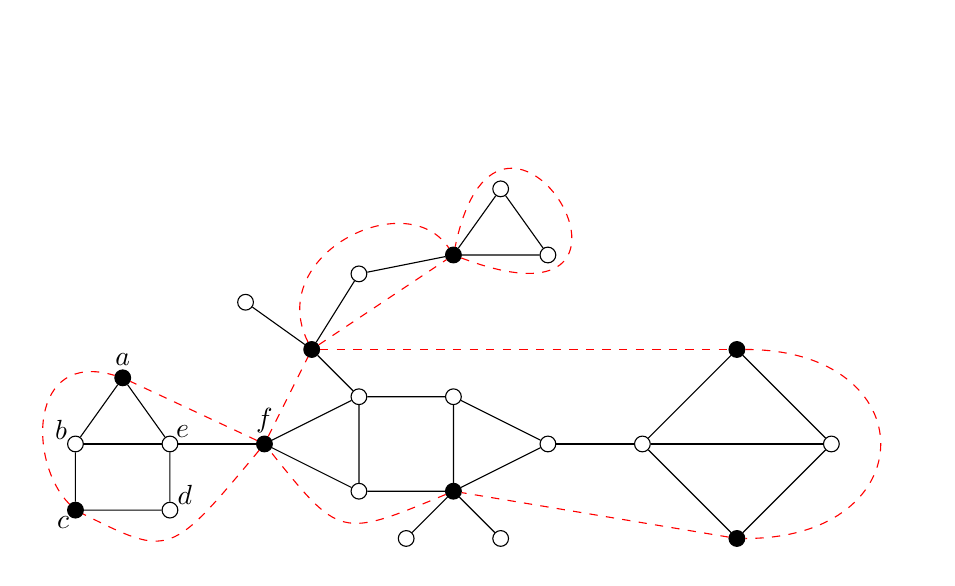
\begin{tikzpicture}[scale=1.2,auto=left]
    
%     \node[style={text=black}] at (-1.5,0) {$H$};
    
    \begin{scope}[every node/.style={circle,draw=black,fill=white,minimum size=0.2cm, inner sep=0}]
      \node[fill=black,label=91:$f$] (a) at (0,0) {};
      \node[] (b) at (1,0.5) {};
      \node[] (c) at (2,0.5) {};
      \node[] (d) at (3,0) {};
      \node[fill=black] (e) at (2,-0.5) {};
      \node[] (f) at (1,-0.5) {};
      \node[] (g) at (4,0) {};
      \node[fill=black] (h) at (5,1) {};
      \node[] (i) at (6,0) {};
      \node[fill=black] (j) at (5,-1) {};
      \node[label=45:$e$] (k) at (-1,0) {};
      \node[label=45:$d$] (l) at (-1,-0.7) {};
      \node[fill=black,label=-135:$c$] (m) at (-2,-0.7) {};
      \node[label=135:$b$] (n) at (-2,0) {};
      \node[fill=black,label=90:$a$] (o) at (-1.5,0.7) {};
      \node[fill=black] (p) at (0.5,1) {};
      \node[] (q) at (-0.2,1.5) {};
      \node[] (r) at (1,1.8) {};
      \node[] (s) at (1.5,-1) {};
      \node[] (t) at (2.5,-1) {};
      
      \node[fill=black] (u) at (2,2) {};
      \node[] (v) at (3,2) {};
      \node[] (w) at (2.5,2.7) {};
      
      \foreach \from/\to in {a/b,b/c,c/d,d/e,e/f,f/a,f/b,c/e,
                             d/g,g/h,h/i,i/j,j/g,g/i,
                             a/k,k/l,l/m,m/n,n/o,o/k,k/n,
                             e/t,e/s,  b/p,p/q,p/r,
                             r/u,u/v,v/w,w/u}
	\draw (\from) -- (\to);
	
      \foreach \from/\to in {a/p,p/h,j/e,a/o,p/u}
	\draw[dashed,red] (\from) -- (\to);
	
       \draw[dashed,red] (h) .. controls (7,1) and (7,-1) .. (j);
       \draw[dashed,red] (e) .. controls (0.8,-1) .. (a);
       \draw[dashed,red] (a) .. controls (-1,-1.2) .. (m);
       \draw[dashed,red] (m) .. controls (-2.5,-0.2) and (-2.5,1) .. (o);
       \draw[dashed,red] (p) .. controls (0,2) and (1.5,2.75) .. (u);

       \draw[dashed,red] (u) .. controls (4.5,1.05) and (2.5,4.4) .. (u);
	
%       \draw[dotted] (u) .. controls (-0.5,2.5) and (1.7,2.2) .. (w);
%       
      
    \end{scope}
  \end{tikzpicture}
  
  \caption{An outerplane graph $G$ with blocking set $B$ (denoted in black). The edges of $\block_{B}(G)$ are denoted in dashed. (WARNING: Three self-loops are missing. Next time, make some legs black.}
  \label{fig:blocking_graph}
  
  \end{figure}

The fact that a blocking set does not contain both endpoints of any
chord of $G$ (\obsref{no-chords}) implies the following observation:

\begin{obs}\obslabel{cactus}
   For every outerplane graph $G$ and any blocking set $B$ of $G$,
   the blocking graph $\block_B(G)$ is a bridgeless cactus graph.
\end{obs}

In the previous section, we sketched a proof of an upper bound of
8 on the facial chromatic number of biconnected outerplane graphs.
This proof works by non-repetitively 4-colouring the tree, $G\setminus B$, obtained after removing the blocking set and then non-repetiviely
4-colouring a cycle, $C$, of vertices in the blocking set.  This cycle,
$C$, is actually the blocking graph, $\block_B(G)$.  The following lemma
shows that this strategy generalizes to the situation where we can find
a facial non-repetitive colouring of $\block_B(G)$ with few colours.

\begin{lem}\label{lem:hitting_plus_four}
  Let $G$ be an outerplane graph and $B$ be a blocking set of $G$. If
  there exists a facial nonrepetitive $k$-colouring of (the outside
  face of) $\block_{B}(G)$, then there exists a facial nonrepetitive
  $(4+k)$-colouring of $G$.
\end{lem}

\begin{proof}
  Argue separately about paths in the inner faces and outer face.  Note:
  Take special care that we don't say anything incorrect about self-loops.
\end{proof}

Discuss the difficulty of colouring blocking graphs with odd-cycles.

\subsection{Colouring Even Cactus Graphs}

\begin{lem}
   For every cactus graph, $G$, with no odd cycles, $\pi_f(G)\le 7$.
\end{lem}

\begin{proof}
   Copy from Lucas.
\end{proof}

\subsection{Making an Even Blocking Graph}

\begin{lem}\lemlabel{even-biconnected}
  For every biconnected outerplane graph, $G$, and any vertex $v\in V(G)$:
  \begin{itemize}
    \item $G$ has a blocking set $B$ such that $\block_B(G)$ is an even cycle 
       and $v\in B$; and
    \item $G$ has a blocking set $B$ such that $\block_B(G)$ is an even cycle 
       and $v\not\in B$.
  \end{itemize}
\end{lem}

\begin{proof}
  We first obtain a blocking set $B'$ that contains or does not
  contain $v$, as appropriate, by applying \lemref{biconnected} or
  \corref{biconnected-out}. It is simple to verify that $\block_{B'}(G)$
  is a cycle;  if it is an even cycle, then we are done, so we may assume
  that $\block_{B'}(G)$ is an odd cycle.

  If $G$ has only one internal face, then $B'$ contains one vertex,
  $u$, on this face and $\block_{B'}(G)$ is an odd cycle (of length 1).
  In this case, we can select the neighbour, $w$, of $u$ such that
  $w\neq v$ and let $B=B'\cup\{w\}$.  It is easy to verify that $B$ is
  a blocking set, and either includes or excludes $v$, as appropriate,
  and that $\block_B(G)$ is a 2-cycle.

  Thus, we may assume that $G$ has at least two internal faces and we
  consider several cases:
 
  \begin{enumerate}
  \item If $G$ contains an ear, $F$, with four or more vertices such
  that either $v\not\in V(F)$ or $v$ is one of the endpoints of the
  chord of $F$. There is exactly one vertex $x\in B'$ on the face $F$.
  Let $y$ be a neighbour of $x$ such $y$ is not on the chord of $F$
  (so $y$ has degree 2). Such a $y$ exists since $F$ has at least four
  vertices.  Set $B=B'\cup \{y\}$.  Now $|B|$ is even, so $\block_B(G)$
  is an even cycle.  Furthermore, $G\setminus B'$ is a tree and $y$
  is a leaf in this tree, so $G\setminus B$ is also a tree.  Finally,
  by choice, $B$ contains $v$ if and only if $B'$ contains $v$, so $B$
  satisifies the conditions of the lemma.

  \item Next, consider the case where $G$ contains triangular ear, $F$,
  such that one of the endpoints of the chord of $F$ is in $B'$ and $v$
  is not the degree 2 vertex, $y$, of $F$.  By the same argument as above,
  $B=B'\cup\{y\}$ satisfies the conditions of the lemma, so we are done.

  \item 
  For an edge $uw\in E(G)$, let $V_{uw}'$ and $V_{uw}''$ be the two
  (possibly empty) sets of vertices in the two connected components
  of $G\setminus\{u,w\}$.  Let $G_{uw}'=G[V_{uw}'\cup\{u,w\}]$ and
  $G_{uw}''=G[V_{uw}''\cup\{u,w\}]$.

  If neither of the two previous cases applies, then there exists an edge
  $uw$ of $G$ such that $v\not\in V_{uw}'$ and the weak dual of $G_{uw}'$
  is a star whose central vertex is the face, $F_{uw}$ incident on $uw$.
  (Note that $v$ may be one of $u$ or $w$.)

  We will now show that we can select another vertex, $y$, from
  $V_{uw}'\setminus B'$ so that $B=B'\cup\{y\}$ is a blocking set.
  This is sufficient since $|B|$ is even so $\block_B(G)$ is an even
  cycle.  

  \begin{itemize}
  \item[$(\star)$]
  By choice, $G_{uw}'$ has at least 2 faces and each of them, other
  than $F_{uw}$, is a triangular ear incident to $F_{uw}$ and whose
  degree-2 vertex is in $B'$ (otherwise, one of those faces would have
  been handled by Case~1 or 2).
  \end{itemize}

  Let $x$ be the unique vertex of $B'$ on $F_{uw}$. The vertex $x$ has two
  neighbours on $F_{uw}$.  We claim that one of these is not in $\{u,w\}$
  and we take this vertex to be $y$.  This claim is valid because
  otherwise, $F_{uw}$ is a triangle, $xuw$, with $x\not\in\{u,w\}$.
  This case is not possible because by $(\star)$ at least one of $xu$ or
  $xw$ is incident on both $F_{uw}$ and a triangular ear $E$ of $G_{uw}'$.
  Both $x$ and the degree 2 vertex of $E$ are in $B'$.  This contradicts
  the fact that $B'$ includes at most one vertex from each face of $G$,
  including $E$.

  Let $B=B'\cup\{y\}$.  We claim that $B$ is a blocking set of $G$.
  First, note that $B$ contains at most two vertices from each face, $F$,
  of $G$, so $F\setminus B'\neq \emptyset$.  We now show that $y$ is a
  leaf in the tree $G\setminus B'$, so that $G\setminus B$ is also a tree.

  First, observe that $xy$ is not a chord of $G$ since, by $(\star)$,
  the face incident to $xy$ other than $F_{uw}$ would have two of its
  vertices in $B'$.  Thus, in addition to $x$, $y$ has at most two
  neighbours in $G$.  One of these, $z$, is on $F_{uw}$ and $z\neq x$
  so $z\notin B'$.  Finally, $y$ may have one additional neighbour,
  which is a degree-2 vertex of a triangular ear incident on $yz$.
  In this case, by $(\star)$, this degree-2 vertex is in $B'$.  Thus,
  $yz$ is the only edge incident to $y$ in the tree $G\setminus B'$
  so $y$ is a leaf in this tree. \qedhere
\end{enumerate}
\end{proof}

\begin{lem}\lemlabel{even-bridgeless}
  Every simple bridgeless outerplane graph $G$ has a blocking set $B$ such that
  all cycles in $\block_B(G)$ are even. 
\end{lem}

\begin{proof}
  The proof is by induction on the number of 2-connected components
  of $G$.  If $G$ has no 2-connected components, then we take $B$ to be
  the empty blocking set.  If $G$ has only one 2-connected component,
  then we apply \lemref{even-biconnected}.
  Otherwise, select a 2-connected component, $C$, that
  shares exactly one vertex, $v$, with the rest of $G$.  Let
  $G'=G\setminus(V(C)\setminus\{v\})$ and apply induction on $G'$
  to obtain a blocking set, $B'$, of $G'$ such that $\block_{B'}(G')$
  has only even cycles.  There are two cases to consider:
  \begin{enumerate}
    \item If $B'$ contains $v$, then we apply the first part of
    \lemref{even-biconnected} to obtain a blocking set $B''$ of $C$
    such that $\block_{B''}(C)$ is an even cycle and $v\in B''$.  We take
    $B=B'\cup B''$, which clearly forms a blocking set of $G$.  
    The blocking graph $\block_B(G)$ is simply the union of the
    two blocking graphs $\block_{B'}(G)$ and $\block_{B''}(C)$, which have
    only the vertex $v$ in common.  Thus, every cycle in $\block_B(G)$
    is also a cycle in one of these two graphs, so it has even length.

    \item If $B'$ does not contain $v$, then we apply the second part
    of \lemref{even-biconnected} to obtain a blocking set $B''$ of $C$
    such that $\block_{B''}(C)$ is an even cycle and $v\not\in B''$.
    We take $B=B'\cup B''$.

    Starting at some vertex appropriate vertex in $V(G)\setminus V(C)$ 
    in the facial walk
    on the outer face of $G$, there is a last vertex, $x\in V(G')\cap B'$,
    encountered before the walk encounters the first vertex $v\in V(C)\cap
    B''$ and there is a last vertex $w\in V(C)\cap B''$ encountered
    before the walk returns to the next vertex $y\in V(G')\cap B'$.
    The edge $xy$ is in $\block_{B'}(G')$ and the edge $vw$ is in
    $\block_{B''}(C)$.  

    Since every blocking graph is a bridgeless cactus graph
    (\obsref{cactus}), each of these edges is part of one even cycle
    in its respective graph. In $\block_{B}(G)$ these two cycles are
    merged by removing the edges $xy$ and $vw$ and adding the edges
    $xv$ and $yw$.  The resulting cycle is even.  Every other cycle
    in $\block_B(G)$ is also a cycle in one of $\block_{B'}(G')$ or
    $\block_{B''}(C)$ so it has even length. \qedhere
  \end{enumerate}
\end{proof}

\begin{lem}\lemlabel{even}
  Every simple outerplane graph $G$ has a blocking set $B$ such that all cycles
  in $\block_B(G)$. 
\end{lem}

\begin{proof}
  The proof is by induction on the number of bridges of $G$.  If $G$
  has no bridges, then we apply \lemref{even-bridgeless}.  Otherwise,
  select some bridge $uw$ of $G$ and contract it to obtain a graph $G'$
  in which $uw$ corresponds to a single vertex $v$.  By induction,
  we obtain a blocking set $B'$ of $G'$ such that $\block_{B'}(G')$
  has only even cycles (or is empty).  There are two cases to consider:
  \begin{enumerate}
    \item If $v\in B'$, then we take $B=B'\cup\{u,w\}\setminus\{v\}$. This introduces exactly one new cycle in $\block_B(G)$ that is not present in $\block_{B'}(G')$ and this cycle has length 2.

    \item If $v\not\in B'$, then we take $B=B'$, so
    $\block_B(G)=\block_{B'}(G')$. \qedhere
  \end{enumerate}
\end{proof}


\bibliographystyle{plainurl}
\bibliography{arraylayouts}

\end{document}


